\chapter{シミュレーションにおける実験評価}\label{simulation}

この章では,実験が適切に構築されていることをMonte Carloシミュレーションを用いて評価する.
また,期待されるスペクトルを推定する.

\section{シミュレーションの意義}

我々の実験では,複雑に物体が組み合わされており,我々が求めるイベントがどれくらいの頻度で発生しうるのかを計算するのは立体角や断面積の計算が入り組みかなり難しい.
そこでMonte Carloシミュレーションを用いて,実験レートを評価する.本実験では,Monte CarloシミュレーションとしてGeant4を用いてプラスチックシンチレータの中で停止せずに陽電子がターゲットに到達するか,そしてターゲットから発生したガンマ線がNaIシンチレータでエネルギーを落とすかを確かめた.
また,実験でのバックグラウンドを推定した.

今回用いた線源は$\ce{^{22}Na}$ の標準線源であり,200 kBqのものである.

この線源強度と我々の実験期間約1週間を考慮して,1 Hzの実験レートとS/N比100を目標に実験のデザインが適当か検証した.

線源の$\beta$崩壊から考えると実験の各過程はごく稀なイベントであり,一度に全てのジオメトリを実装して実験を行うのは効率が悪い.
今回は本実験でオルソポジトロニウムの寿命を測定する過程の評価を,$\ce{^{22}Na}$ 線源が$\beta$ 崩壊した陽電子がシンチレーターを通過してシリカゲルに到達する過程のレート評価,線源から直接NaIシンチレータに入る$\gamma$ 線の評価,そして形成されたポジトロニウムが崩壊し,放出された$\gamma$ 線がNaIシンチレータで落とすエネルギーの評価の3つに分割してシミュレーションを行った.
これらを統合して考える事で効率よく適切な評価を行うことができる.
プログラムの実装の都合上,シミュレーション結果に関係の無い\ce{^{22}Na}の寿命のみ,付属のライブラリを書き換えた.

\section{プラスチックシンチレーターの通過}
\label{plastic_scintillator_effect}

\subsection{概要}
今回の実験で用いられたプラスチックシンチレータは0.15 mmの厚みのものである.線源から放出される陽電子が,シンチレータ内で停止してしまうとシリカゲルに到達せずポジトロニウムを形成することができない.
ポジトロニウムを形成するためには,陽電子がまず標準線源の0.1mmの厚みのアルミ窓を通過して,空気中を伝播し,さらにシンチレータをエネルギーを落としきること無く通過する必要がある.
実際の線源を忠実に再現したジオメトリを作成し,シンチレータと線源の距離を変えながら通過してくる粒子の割合を調べた.

このとき,ポジトロニウムのミキシングを起こすために用いる磁場0.1Tは,陽電子をシリカゲルまで導く方向になるよう設定した.実際の実験でもこの方向に磁場を使用することが可能である.

\subsection{ジオメトリ}

\begin{figure}[htbp]
	\centering
		\includegraphics[width=10cm]{img/test1_geometry.pdf}
	\caption{構築したジオメトリ}
	\label{test1_geometry}
\end{figure}

図\ref{test1_geometry} はプラスチックシンチレーターの試験として作成したジオメトリで,標準線源とその表面から距離$d$ mm離れたターゲットである$\phi8$ mm,厚み0.15 mmのプラスチックシンチレーター(赤),その直後に置かれた理想的な粒子検出器で構成されている.
緑の線で示されているのが$\gamma$線,青の線で示されているのが陽電子の軌跡である.図では試しに\ce{^{22}Na}が100個崩壊した軌跡を表示している.
標準線源はデータシートにしたがって作成し,アクリルのケースと0.1 mm厚のアルミニウム製の窓を実装してある.理想的な粒子検出器は入射した粒子の種類とエネルギーが分解能無限大で確実にわかる.
\ce{^{22}Na}はbranching ratioにしたがって$\beta^+$崩壊する.

\subsection{陽電子到達数と立体角}

プラスチックシンチレーターを線源から遠くに置くほど,透過する陽電子数は減少すると考えられる.この減少には,空気中を伝播する際に陽電子が相互作用することも影響すると考えられるが,大部分の影響は立体角の減少に由来すると予想される.今回は理想的な粒子検出器を実装しているため,ニュートリノの数を調べることでも立体角を概算する事ができる.無論,立体角$\Omega$srを解析的に計算することも可能で,

\begin{equation}
	\Omega = 2\pi \left( 1-\cos\left(\arctan\frac{8/2}{d+2.5}\right)\right)
\end{equation}

で与えられる.今回は$d$を線源の表面からシンチレーターを通過するまでの距離と定義しているので,放射線源中心からの補正2.5 mmを加えている.

\subsection{磁場の援用}
概要でも触れたが,ポジトロニウムのミキシングを起こさせるための磁場を,陽電子をターゲットまで導くことにも援用することができる.
強力に磁場方向に引き寄せられるのが見て取れるので,磁場をかけたとき,かけないときでレートを比較する.

\subsection{結果}

図\ref{test1}は$d=100$mmで,100Mイベント生成した際のシンチレーターを通過した陽電子のエネルギースペクトル(青)である. シンチレーターを外したとき(赤)と比較した.
また,図\ref{scinti_test}がシンチレーターを陽電子が通過する割合の距離依存である.磁場をかけたとき(赤)と磁場をかけていないとき(青)をプロットし,計算された立体角に定数を乗じて$d=10$mmの磁場なしの点と重なるようにプロットした.

\begin{figure}[htbp]
	\centering
		\includegraphics[width=10cm]{fig/test1.pdf}
	\caption{シンチレータを透過した陽電子のエネルギー}
	\label{test1}
\end{figure}


\begin{figure}[htbp]
	\centering
		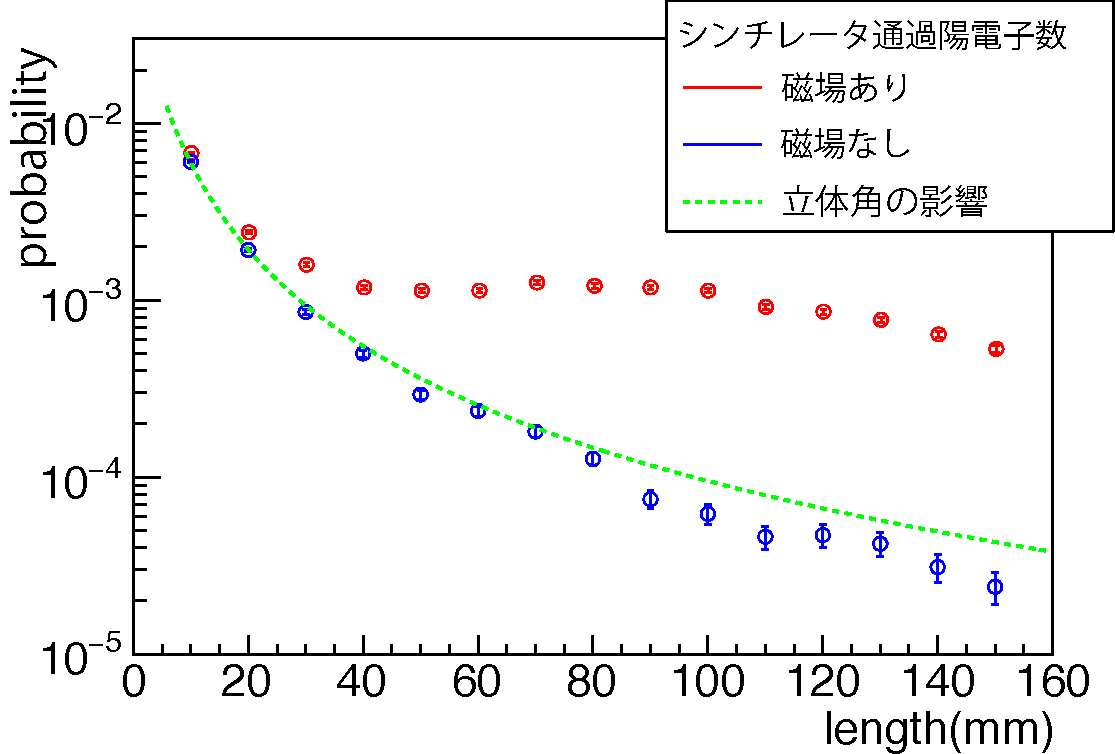
\includegraphics[width=10cm]{fig/scinti_test.pdf}
	\caption{プラスチックシンチレータ通過粒子割合}
	\label{scinti_test}
\end{figure}

\subsection{考察}

結果\ref{test1}では,シンチレータを通過してきた陽電子のエネルギースペクトルを再現している.プラスチックシンチレータでおよそ40\%程度陽電子を損失するが,約1/1000の陽電子が到達し実験に十分な陽電子が通過していると判断する.

一方で,磁場をかけたときとかけていないときで,陽電子の到達数には差がある,
磁場の無いときは陽電子数は距離が伸びるにつれてほぼ立体角に従い減り続けていくが,磁場のある際には40-110 mm程度まで陽電子数に大きな変化がない.この結果より実際の設計ではターゲットであるシリカゲルまで100 mm程度線源から離した.線源から出る$\gamma$線が直接NaI(Tl)シンチレーターに入らないように遮蔽することを考えるとシンチレーターの極近くに線源を置くことは現実的ではないため,できる限り離れつつもレートを確保することをねらったためである.

\begin{figure}[htbp]
	\centering
		\includegraphics[width=10cm]{img/test1b_geometry.pdf}
	\caption{実装した鉛コリメータ}
	\label{test1b_geometry}
\end{figure}

\begin{figure}[htbp]
	\centering
		\includegraphics[width=10cm]{fig/collimator_loss.pdf}
	\caption{鉛コリメータで失われる陽電子}
	\label{collimator_loss}
\end{figure}

\section{線源からのバックグラウンド評価}

第\ref{plastic_scintillator_effect}節で,プラスチックシンチレータの評価で,ターゲットであるシリカゲルに到達する陽電子数について定量的に見積もることができた.
次に我々の求めている事象に対して,バックグラウンドとなる線源から直接出る$\gamma$線がどのくらい多いのかを評価する.


\subsection{ジオメトリ}
実際の実験装置とほとんど同じジオメトリを構築し,シミュレーションを行った.

\begin{figure}[htbp]
	\centering
		
\includegraphics[width=10cm]{img/test2_geometry.pdf}
	\caption{構築したジオメトリ}
	\label{test2_geometry}
\end{figure}

\subsection{イベントバックグラウンド比}

\begin{figure}[htbp]
	\centering
		\includegraphics[width=10cm]{fig/test2.pdf}
	\caption{カット前のイベントとバックグラウンド}
	\label{test2}
\end{figure}

\subsection{陽電子停止位置}

\begin{figure}[htbp]
	\centering
		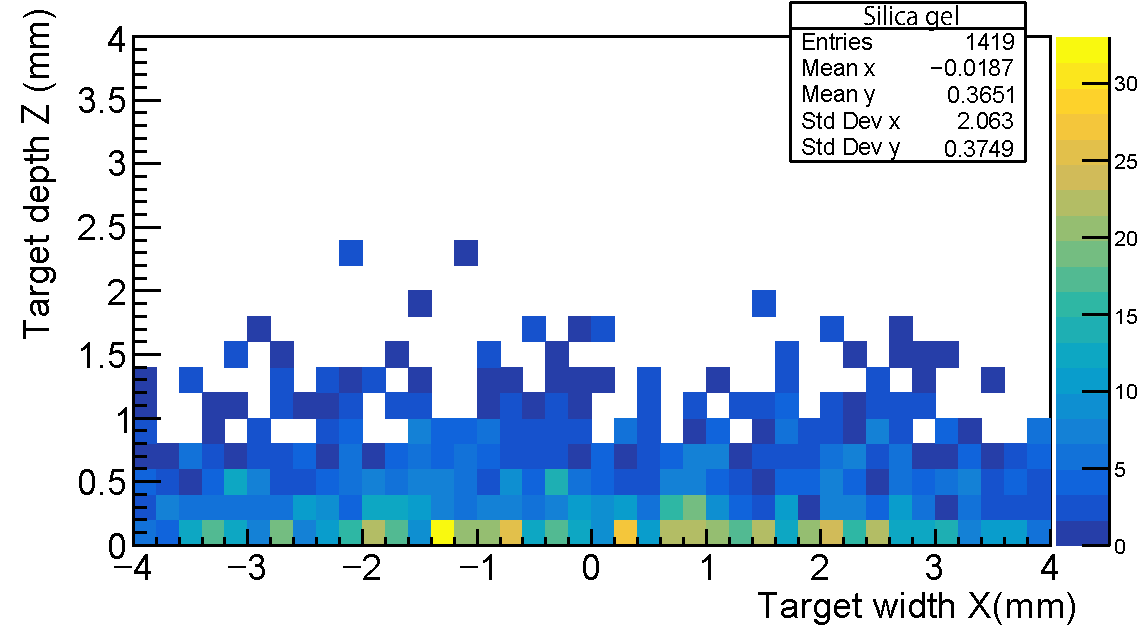
\includegraphics[width=10cm]{fig/test2bXY.pdf}
	\caption{停止方向X-Y方向}
	\label{test2bXY}
\end{figure}

\begin{figure}[htbp]
	\centering
		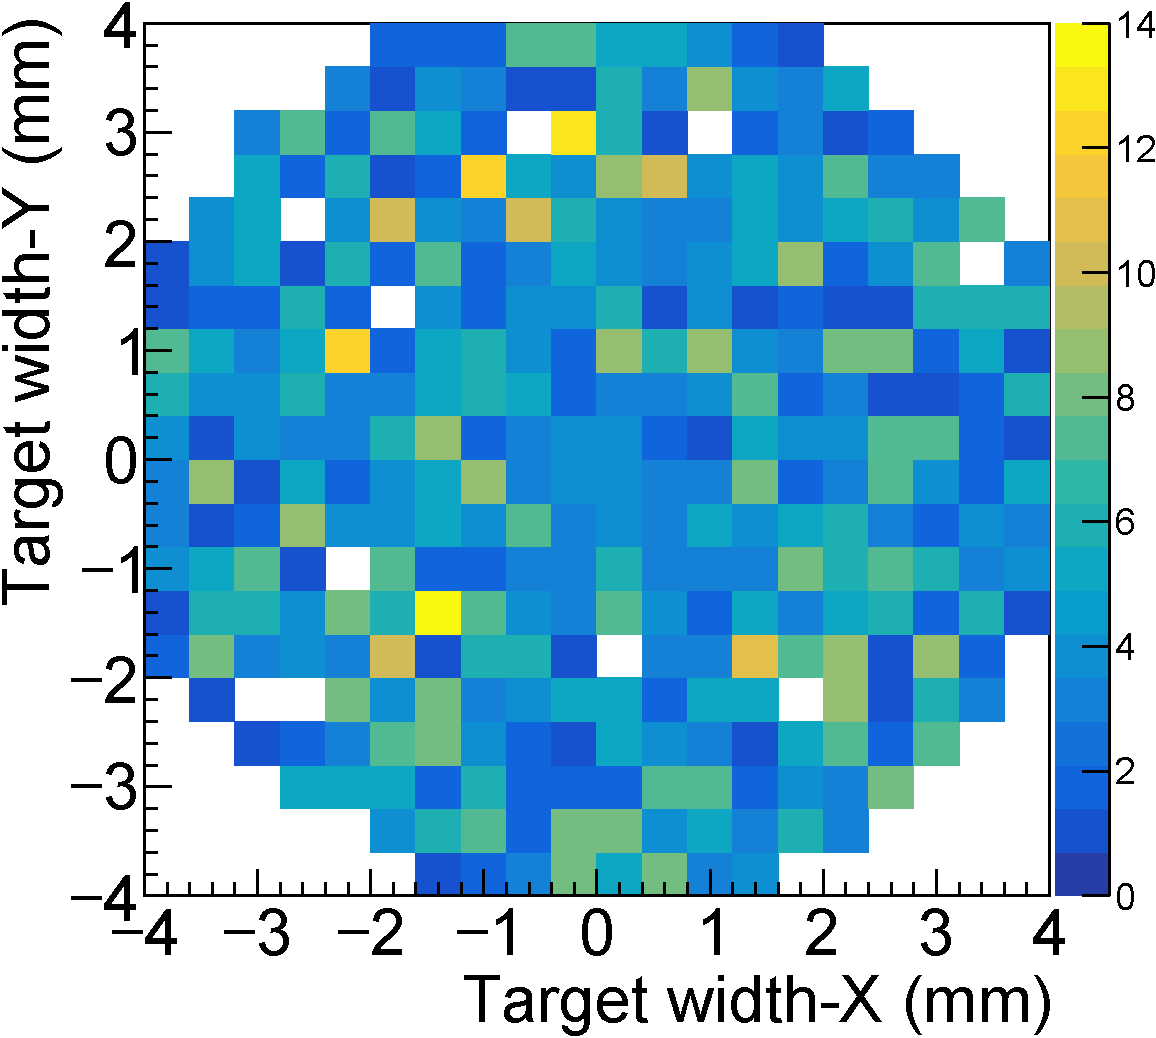
\includegraphics[width=7cm]{fig/test2bYZ.pdf}
	\caption{停止位置Y-Z方向}
	\label{test2bYZ}
\end{figure}

\subsection{考察}


\section{予想されるエネルギースペクトル}

\subsection{初期粒子発生}
先だって行った2つのシミュレーションにより,我々の実験でのイベント頻度が概算された.最後に,この実験によって実際にどのような物理量が得られるべきか検討する.
公式にリリースされているGeant4にはポジトロニウムの様なエキゾチック原子の挙動は含まれておらず,前項でのシミュレーションでは陽電子はシリカゲル中で2$\gamma$崩壊していた.そこでポジトロニウムの崩壊を実装した.
実際にはスピン交換反応や,ピックオフ反応が起こり,実際に入射した陽電子がどのくらいの確率でオルソポジトロニウムを形成するのか理論的な予測は不可能であるため,$2\gamma$に崩壊する事象と$3\gamma$に崩壊する事象を分けてシミュレーションを行う.

\subsection{結果}

\begin{figure}[htbp]
	\begin{tabular}{cc}

	\centering
		\begin{minipage}{0.5\hsize}
		\includegraphics[width=7cm]{fig/gamma2.pdf}
	\caption{$2\gamma$崩壊のスペクトル}
	\label{gamma2}
		\end{minipage}&

		\begin{minipage}{0.5\hsize}
	\centering
		\includegraphics[width=7cm]{fig/gamma3.pdf}
	\caption{$3\gamma$崩壊のスペクトル}
	\label{gamma3}
		\end{minipage}

		\end{tabular}
\end{figure}

\subsection{考察}


\section{実験評価のまとめ}

\subsection{結果}
以上の各評価を統合して,実験レートとバックグラウンドレートを推定する,

\begin{figure}[htbp]
	\centering
		\includegraphics[width=10cm]{fig/test_all.pdf}
	\caption{1週間の測定で期待されるスペクトル}
	\label{test_all}
\end{figure}

\subsection{議論}

